% Subsection on buzzer/woofer

Enfin, le dernier composant nécessaire est un \emph{baffle} ou un \emph{buzzer}. Ces éléments sont représentés sur les Figures \ref{fig:woofer_pic} et \ref{fig:buzzer_pic} respectivement. Le rôle de ces composants est de transformer un signal électrique (tension/courant) provenant de l'amplificateur audio, en signal audio (ondes sonores, audibles par nos oreilles humaines). Une capacité de découplage est nécessaire également, entre le baffle/buzzer et l'amplificateur audio, pour éviter de trop large pics de courant qui peuvent endommager l'amplificateur.\\

\begin{minipage}[c]{0.45\textwidth}
	\centering
	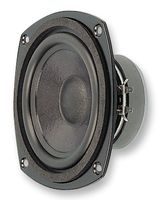
\includegraphics[width=0.4\textwidth]{figures/woofer_picture.jpg}
	\captionof{figure}{Image d'un baffle.}
	\label{fig:woofer_pic}
\end{minipage}
\hfill
\begin{minipage}[c]{0.45\textwidth}
	\centering
	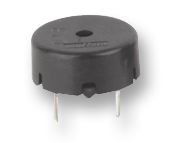
\includegraphics[width=0.4\textwidth]{figures/buzzer_picture.jpg}
	\captionof{figure}{Image d'un buzzer.}
	\label{fig:buzzer_pic}
\end{minipage}
\vspace{1cm}